%!TEX program = xelatex
\documentclass[a4paper, 11pt]{article} % Font size (can be 10pt, 11pt or 12pt) and paper size (remove a4paper for US letter paper)

%\documentclass{article}
%\usepackage[protrusion=true,expansion=true]{microtype} % Better typography
\usepackage{graphicx} % Required for including pictures
\usepackage{wrapfig} % Allows in-line images
\usepackage{ctex}

\usepackage{mathpazo} % Use the Palatino font
\usepackage[T1]{fontenc} % Required for accented characters
\usepackage{fontspec}
\usepackage{xunicode}
\usepackage{xltxtra} 
\usepackage{amsmath}
\usepackage{geometry}
\usepackage[colorlinks,linkcolor=black]{hyperref}
\geometry{a4paper,scale=0.8}
\linespread{1.05} % Change line spacing here, Palatino benefits from a slight increase by default
%\linespread{0.5}
\makeatletter
\renewcommand\@biblabel[1]{\textbf{#1.}} % Change the square brackets for each bibliography item from '[1]' to '1.'
\renewcommand{\@listI}{\itemsep=0pt} % Reduce the space between items in the itemize and enumerate environments and the bibliography

\renewcommand{\maketitle}{ % Customize the title - do not edit title and author name here, see the TITLE block below

\begin{flushright} % Right align
{\LARGE\@title} % Increase the font size of the title

\vspace{50pt} % Some vertical space between the title and author name

{\large\@author} % Author name
\\\@date % Date

\vspace{10pt} % Some vertical space between the author block and abstract
\end{flushright}
}

%----------------------------------------------------------------------------------------
%	TITLE
%----------------------------------------------------------------------------------------

\title{\textbf{量子信息学}\\ % Title
lec 5} % Subtitle

\author{\textsc{郝琰 516021910721} % Author
\\{\textit{ACM Class,2016}}} % Institution

\date{\today} % Date
\begin{document}
\maketitle
\section{Class 1}
\subsection{Measurement Review}
\begin{itemize}
\item
测得的结果
$$
P(m) = <\psi|M_m^+M_m|\psi>
$$
\item
测量后的状态
$$
|\psi_m> = \frac{M_m|\psi>}{\sqrt{P(m)}}
$$
\item
$$
\lbrace |m>,m = 1,2,3,...\rbrace\quad M_m = |m><m| \quad A = \sum_m \lambda_m|m><m|
$$
\item
$$
\lbrace P_m, m = 1,2,...\rbrace \quad M_m = P_m \quad \sum_mP_m = I \quad A = \sum_m mP_m
$$
\item
若只关心测得的概率,不关心测量后的状态变成什么\\
POVM(positive operator-valued measure)
$$
\lbrace E_m: m = 1,2,...,k \rbrace \quad E_m \geq 0 \quad \sum_m E_m = I
$$
$$
P(m) = <\psi|E_m|\psi>
$$
$$
E_m = M_m^+M_m
$$
同时它也可以进行一些状态上的合并($E_m$为所需的状态集合)
\end{itemize}

\subsection{idea 1: 复合系统(第四条公理)}
$$
U + \mbox{projective measurement} \rightarrow \mbox{generalized measurement}
$$
$$
U|\psi>|0> = \sum_mM_m|\psi>|m>
$$
注:$|0>$ 相当于outcome,是原本在环境之中的一个space,现在把它放到U中。可以把整个的global space 看作
$$
\lbrace U|\psi>|m> \rbrace
$$
$$
U|\psi>^{'}|0> = \sum_mM_m|\psi^{'}>|m>
$$
$$
(U|\psi>^{'}|0>)^TU|\psi>|0>  = <\psi|\psi>
$$
$$
P(m) = \lbrace I^A \bigotimes |m> \rbrace
$$


\subsection{实际的测量}
\subsubsection{推导}
\begin{itemize}
	\item
	$$
	\lbrace P_i, |\psi_i>\rbrace \rightarrow \lbrace P_i , U|\psi_i> \rbrace
	$$
	\item
	\begin{align*}
	P(m) = P(m|\psi_i)p_i & = \sum_i p_i <\psi_i|E_m^+E_m|\psi_i>\\
	& = \sum_ip_itr(<\psi_i|E_m^+E_m|\psi_i>)\\
	& = tr(\sum_i p_i |\psi_i><\psi_i| E_m^+E_m)\\
	& = tr(\rho E_m^+E_m)
	\end{align*}

	$$
	 \rho = \sum_i p_i|\psi_i><\psi_i| \quad \mbox{density operator}
	$$
	$$
	\rho \geq 0 \quad tr\rho = 1 
	$$
	系统状态可以用密度算子等价刻画
\end{itemize}

\subsubsection{性质}
\begin{itemize}
\item
state $\rho$ is positive operator with trace one
$$
\rho = \sum_i p_i\rho_i
$$
\item
$$
\rho \rightarrow U\rho U^+
$$
\item
$$
p(m) = tr(\rho E_m^+E_m)
$$
\item 
$$
\rho_1 \bigotimes \rho_2 ... \bigotimes\rho_n
$$
\end{itemize}

\clearpage
\section{Class 2}
\subsection{idea 3: 应用1}
编码(量子操作),信道,解码(量子测量)

要求正交以精确传递

Alice and Bob 共享一个纠缠态
\begin{figure}[h]
        \centering
        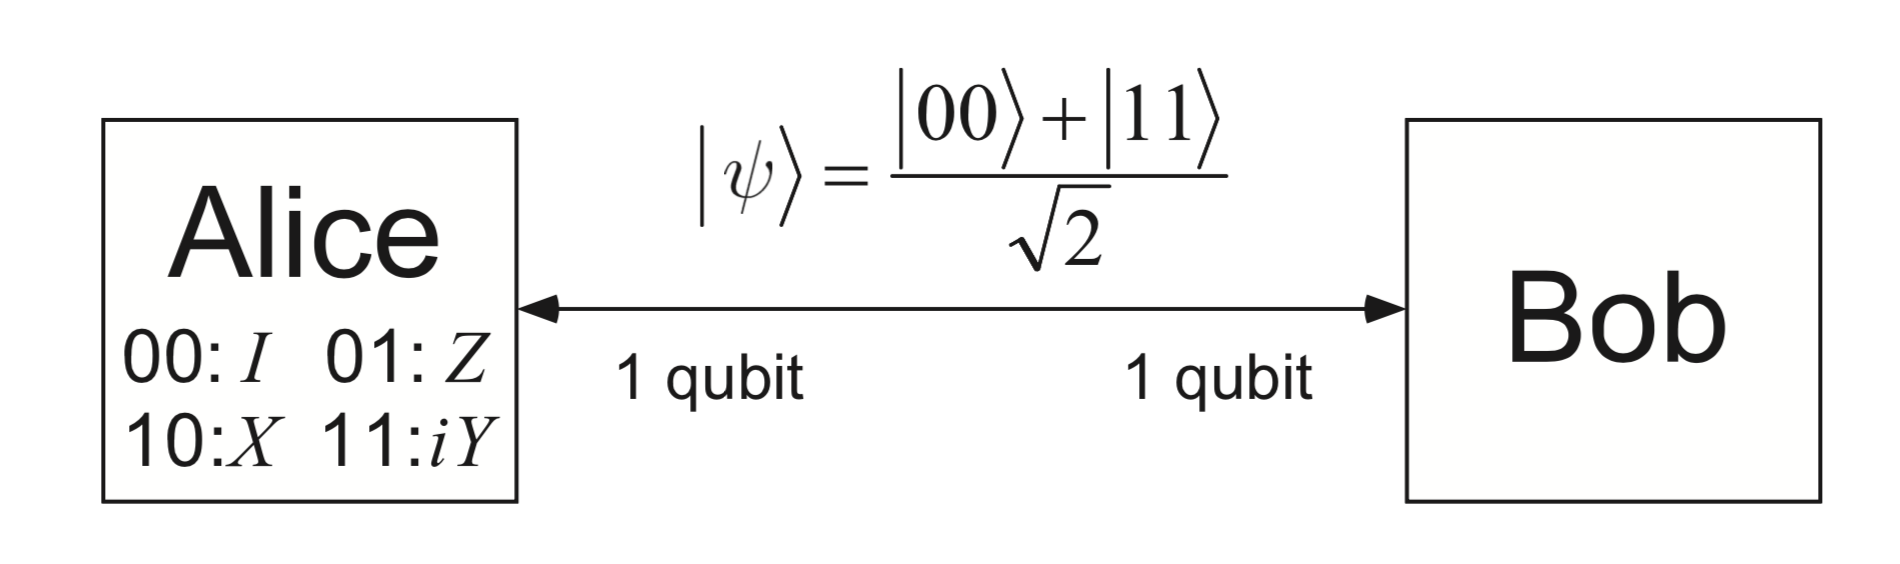
\includegraphics[width=0.99\textwidth]{1}
        \caption{1}
\end{figure}
\begin{figure}[h]
        \centering
        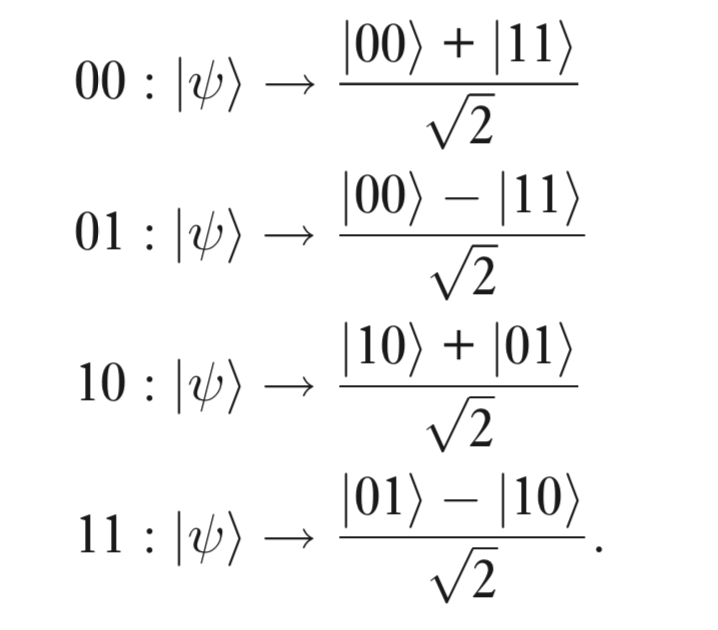
\includegraphics[width=0.5\textwidth]{2}
        \caption{2}
\end{figure}
\subsection{idea 4:如何通过经典信道传量子信息}
Send one qubit to Bob 

要求传递的是状态,而先不管载体如何

Quantum teleportation(1993)

A->B(EPR)
$$
A : |\psi>
$$
\begin{itemize}
	\item
	Alice performs a Bell measurement.
	\item
	Alice sends b0b1 to Bob
	\item
	Bob performs a unitary on this qubit based on b0b1
	$$
	01:I^B \quad 01:X^B \quad 10:Z^B \quad 11:Y^B
	$$
	get
	$$
	\alpha |0> + \beta |1>
	$$
\end{itemize}	
\begin{align*}
&\frac{1}{\sqrt{2}}(\alpha |0>^A + \beta|1>^A)(|0^A0^B>+|1^A1^B>)\\
= & \frac{1}{\sqrt{2}} (\alpha |00>|0>^B+\alpha|01>|1>^B+\beta|10>|0>^B + \beta |11>|1>^B)\\
= & \frac{1}{2}(|\phi_{00}>(\lambda |0> +\beta|1>)^B+|\phi_{01}>(\lambda |1> +\beta|0>)^B+|\phi_{10}>(\lambda |0> -\beta|1>)^B+|\phi_{11}>(\lambda |1> -\beta|0>)^B)
\end{align*}

\subsection{idea 4}
\begin{itemize}
\item
一个judge同时对Alice和Bob做测量,A:Q and R; B:S and T
\item
definite value for Q,R,S,T
\item
for 经典物理学
$$
QS+RS+RT-QT \leq 2
$$
$$
E(QS)+E(RS)+E(RT)-E(QT) \leq 2 
$$
CHSH inequality
\item
for 量子力学
$$
<Q\bigotimes S> + <R\bigotimes S> +<Q\bigotimes T> -<Q\bigotimes T> \leq 2\sqrt{2} 
$$
$$
|\phi> = \frac{|01>- |10>}{\sqrt{2}}
$$
$$
Q = Z^A \quad R = X^A \quad S = \frac{-Z^B - X^B}{\sqrt{2}} \quad T = \frac{Z^B - X^B}{\sqrt{2}}
$$

得到$2\sqrt{2}$

贝尔不等式说明reality or licadity 中至少有一个是不对的

\end{itemize}

\subsubsection*{tail}
$$
|\phi> = \frac{|00> + |11>}{\sqrt{2}} !=|a>|b>
$$
Proof?
$$
\rho^A = \frac{I}{2}
$$
partial trace
$$
tr_B(|a_1><a_2| \bigotimes |b_1><b_2|) = |a_1><a_2|tr(|b_1><b_2|) = |a_1><a_2|(<b_2|b_1>)
$$
$$
\rho^{AB}\quad  \mbox{AB system}
$$
$$
\rho^A = tr_B\rho^{AB} = \sum_i <i^B|\rho^{AB}|r^B>
$$






























\end{document}